% Options for packages loaded elsewhere
\PassOptionsToPackage{unicode}{hyperref}
\PassOptionsToPackage{hyphens}{url}
\PassOptionsToPackage{dvipsnames,svgnames,x11names}{xcolor}
%
\documentclass[
  letterpaper,
  DIV=11,
  numbers=noendperiod]{scrartcl}

\usepackage{amsmath,amssymb}
\usepackage{iftex}
\ifPDFTeX
  \usepackage[T1]{fontenc}
  \usepackage[utf8]{inputenc}
  \usepackage{textcomp} % provide euro and other symbols
\else % if luatex or xetex
  \usepackage{unicode-math}
  \defaultfontfeatures{Scale=MatchLowercase}
  \defaultfontfeatures[\rmfamily]{Ligatures=TeX,Scale=1}
\fi
\usepackage{lmodern}
\ifPDFTeX\else  
    % xetex/luatex font selection
\fi
% Use upquote if available, for straight quotes in verbatim environments
\IfFileExists{upquote.sty}{\usepackage{upquote}}{}
\IfFileExists{microtype.sty}{% use microtype if available
  \usepackage[]{microtype}
  \UseMicrotypeSet[protrusion]{basicmath} % disable protrusion for tt fonts
}{}
\makeatletter
\@ifundefined{KOMAClassName}{% if non-KOMA class
  \IfFileExists{parskip.sty}{%
    \usepackage{parskip}
  }{% else
    \setlength{\parindent}{0pt}
    \setlength{\parskip}{6pt plus 2pt minus 1pt}}
}{% if KOMA class
  \KOMAoptions{parskip=half}}
\makeatother
\usepackage{xcolor}
\setlength{\emergencystretch}{3em} % prevent overfull lines
\setcounter{secnumdepth}{5}
% Make \paragraph and \subparagraph free-standing
\ifx\paragraph\undefined\else
  \let\oldparagraph\paragraph
  \renewcommand{\paragraph}[1]{\oldparagraph{#1}\mbox{}}
\fi
\ifx\subparagraph\undefined\else
  \let\oldsubparagraph\subparagraph
  \renewcommand{\subparagraph}[1]{\oldsubparagraph{#1}\mbox{}}
\fi


\providecommand{\tightlist}{%
  \setlength{\itemsep}{0pt}\setlength{\parskip}{0pt}}\usepackage{longtable,booktabs,array}
\usepackage{calc} % for calculating minipage widths
% Correct order of tables after \paragraph or \subparagraph
\usepackage{etoolbox}
\makeatletter
\patchcmd\longtable{\par}{\if@noskipsec\mbox{}\fi\par}{}{}
\makeatother
% Allow footnotes in longtable head/foot
\IfFileExists{footnotehyper.sty}{\usepackage{footnotehyper}}{\usepackage{footnote}}
\makesavenoteenv{longtable}
\usepackage{graphicx}
\makeatletter
\def\maxwidth{\ifdim\Gin@nat@width>\linewidth\linewidth\else\Gin@nat@width\fi}
\def\maxheight{\ifdim\Gin@nat@height>\textheight\textheight\else\Gin@nat@height\fi}
\makeatother
% Scale images if necessary, so that they will not overflow the page
% margins by default, and it is still possible to overwrite the defaults
% using explicit options in \includegraphics[width, height, ...]{}
\setkeys{Gin}{width=\maxwidth,height=\maxheight,keepaspectratio}
% Set default figure placement to htbp
\makeatletter
\def\fps@figure{htbp}
\makeatother

\usepackage{booktabs}
\usepackage{longtable}
\usepackage{array}
\usepackage{multirow}
\usepackage{wrapfig}
\usepackage{float}
\usepackage{colortbl}
\usepackage{pdflscape}
\usepackage{tabu}
\usepackage{threeparttable}
\usepackage{threeparttablex}
\usepackage[normalem]{ulem}
\usepackage{makecell}
\usepackage{xcolor}
\KOMAoption{captions}{tableheading}
\makeatletter
\@ifpackageloaded{caption}{}{\usepackage{caption}}
\AtBeginDocument{%
\ifdefined\contentsname
  \renewcommand*\contentsname{Table of contents}
\else
  \newcommand\contentsname{Table of contents}
\fi
\ifdefined\listfigurename
  \renewcommand*\listfigurename{List of Figures}
\else
  \newcommand\listfigurename{List of Figures}
\fi
\ifdefined\listtablename
  \renewcommand*\listtablename{List of Tables}
\else
  \newcommand\listtablename{List of Tables}
\fi
\ifdefined\figurename
  \renewcommand*\figurename{Figure}
\else
  \newcommand\figurename{Figure}
\fi
\ifdefined\tablename
  \renewcommand*\tablename{Table}
\else
  \newcommand\tablename{Table}
\fi
}
\@ifpackageloaded{float}{}{\usepackage{float}}
\floatstyle{ruled}
\@ifundefined{c@chapter}{\newfloat{codelisting}{h}{lop}}{\newfloat{codelisting}{h}{lop}[chapter]}
\floatname{codelisting}{Listing}
\newcommand*\listoflistings{\listof{codelisting}{List of Listings}}
\makeatother
\makeatletter
\makeatother
\makeatletter
\@ifpackageloaded{caption}{}{\usepackage{caption}}
\@ifpackageloaded{subcaption}{}{\usepackage{subcaption}}
\makeatother
\ifLuaTeX
  \usepackage{selnolig}  % disable illegal ligatures
\fi
\usepackage{bookmark}

\IfFileExists{xurl.sty}{\usepackage{xurl}}{} % add URL line breaks if available
\urlstyle{same} % disable monospaced font for URLs
\hypersetup{
  pdftitle={Supplementary Material},
  pdfauthor={rachel Robertson and Kelly Cao},
  colorlinks=true,
  linkcolor={blue},
  filecolor={Maroon},
  citecolor={Blue},
  urlcolor={Blue},
  pdfcreator={LaTeX via pandoc}}

\title{Supplementary Material}
\author{rachel Robertson and Kelly Cao}
\date{2024-05-03}

\begin{document}
\maketitle

The supplementary materials include tables and figures from the
exploratory analysis and data analysis that were unused in the final
manuscript.

\begin{figure}[H]

{\centering 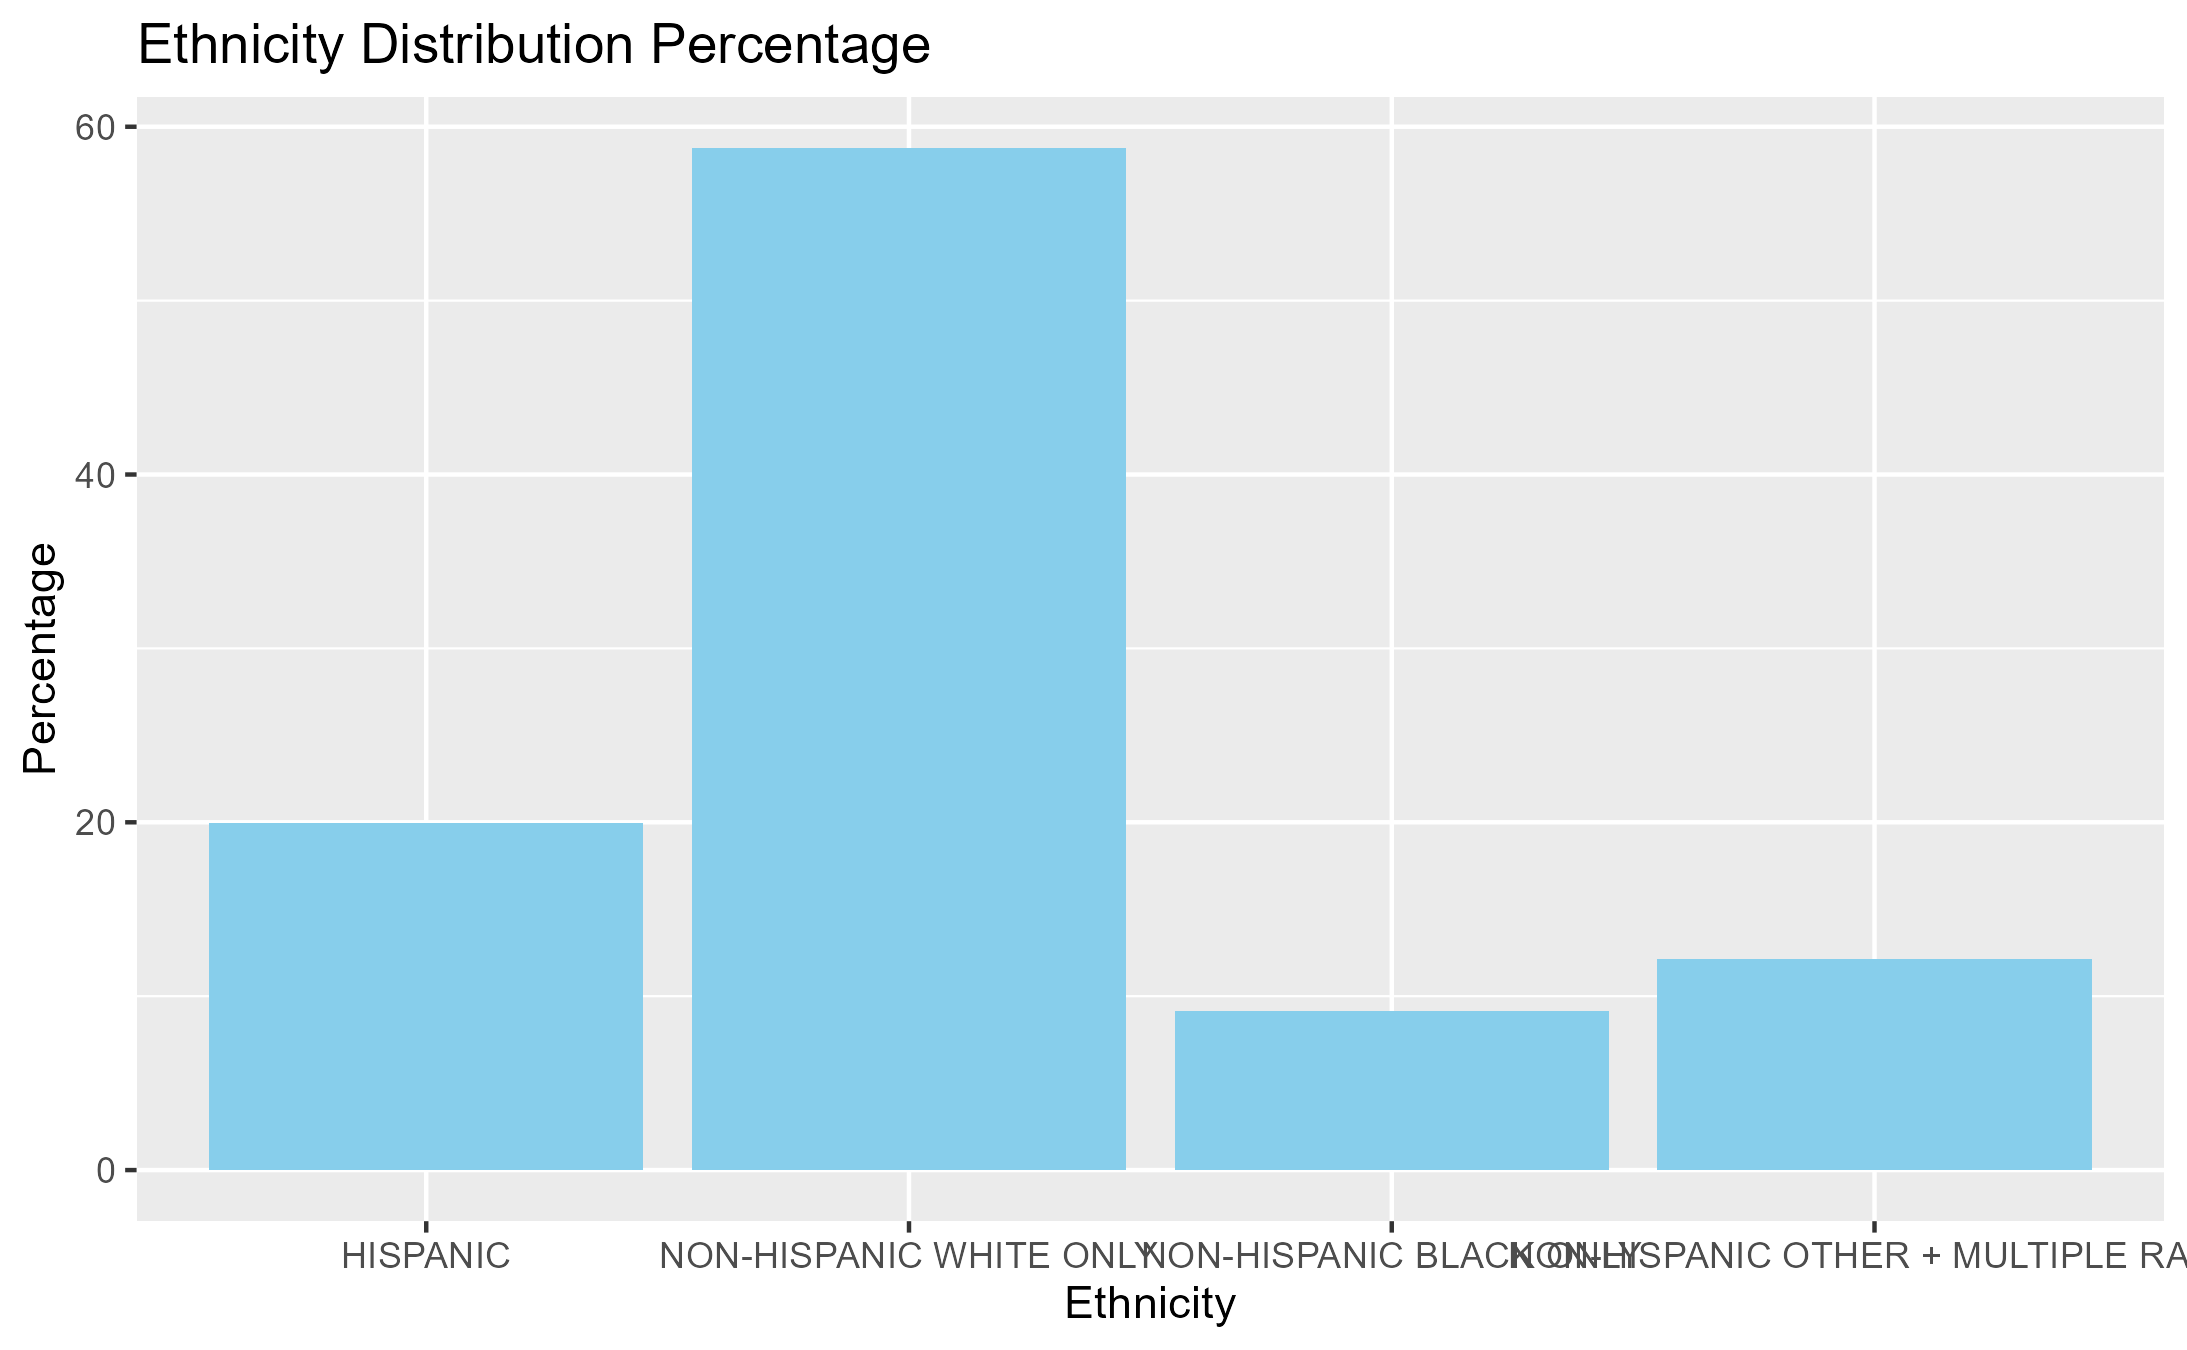
\includegraphics[width=0.8\textwidth,height=\textheight]{../../../results/figures/ethnicity.distribution.png}

}

\caption{S.1. Distribution of ethnicity and race in sample populaiton of
U.S. teens.}

\end{figure}%

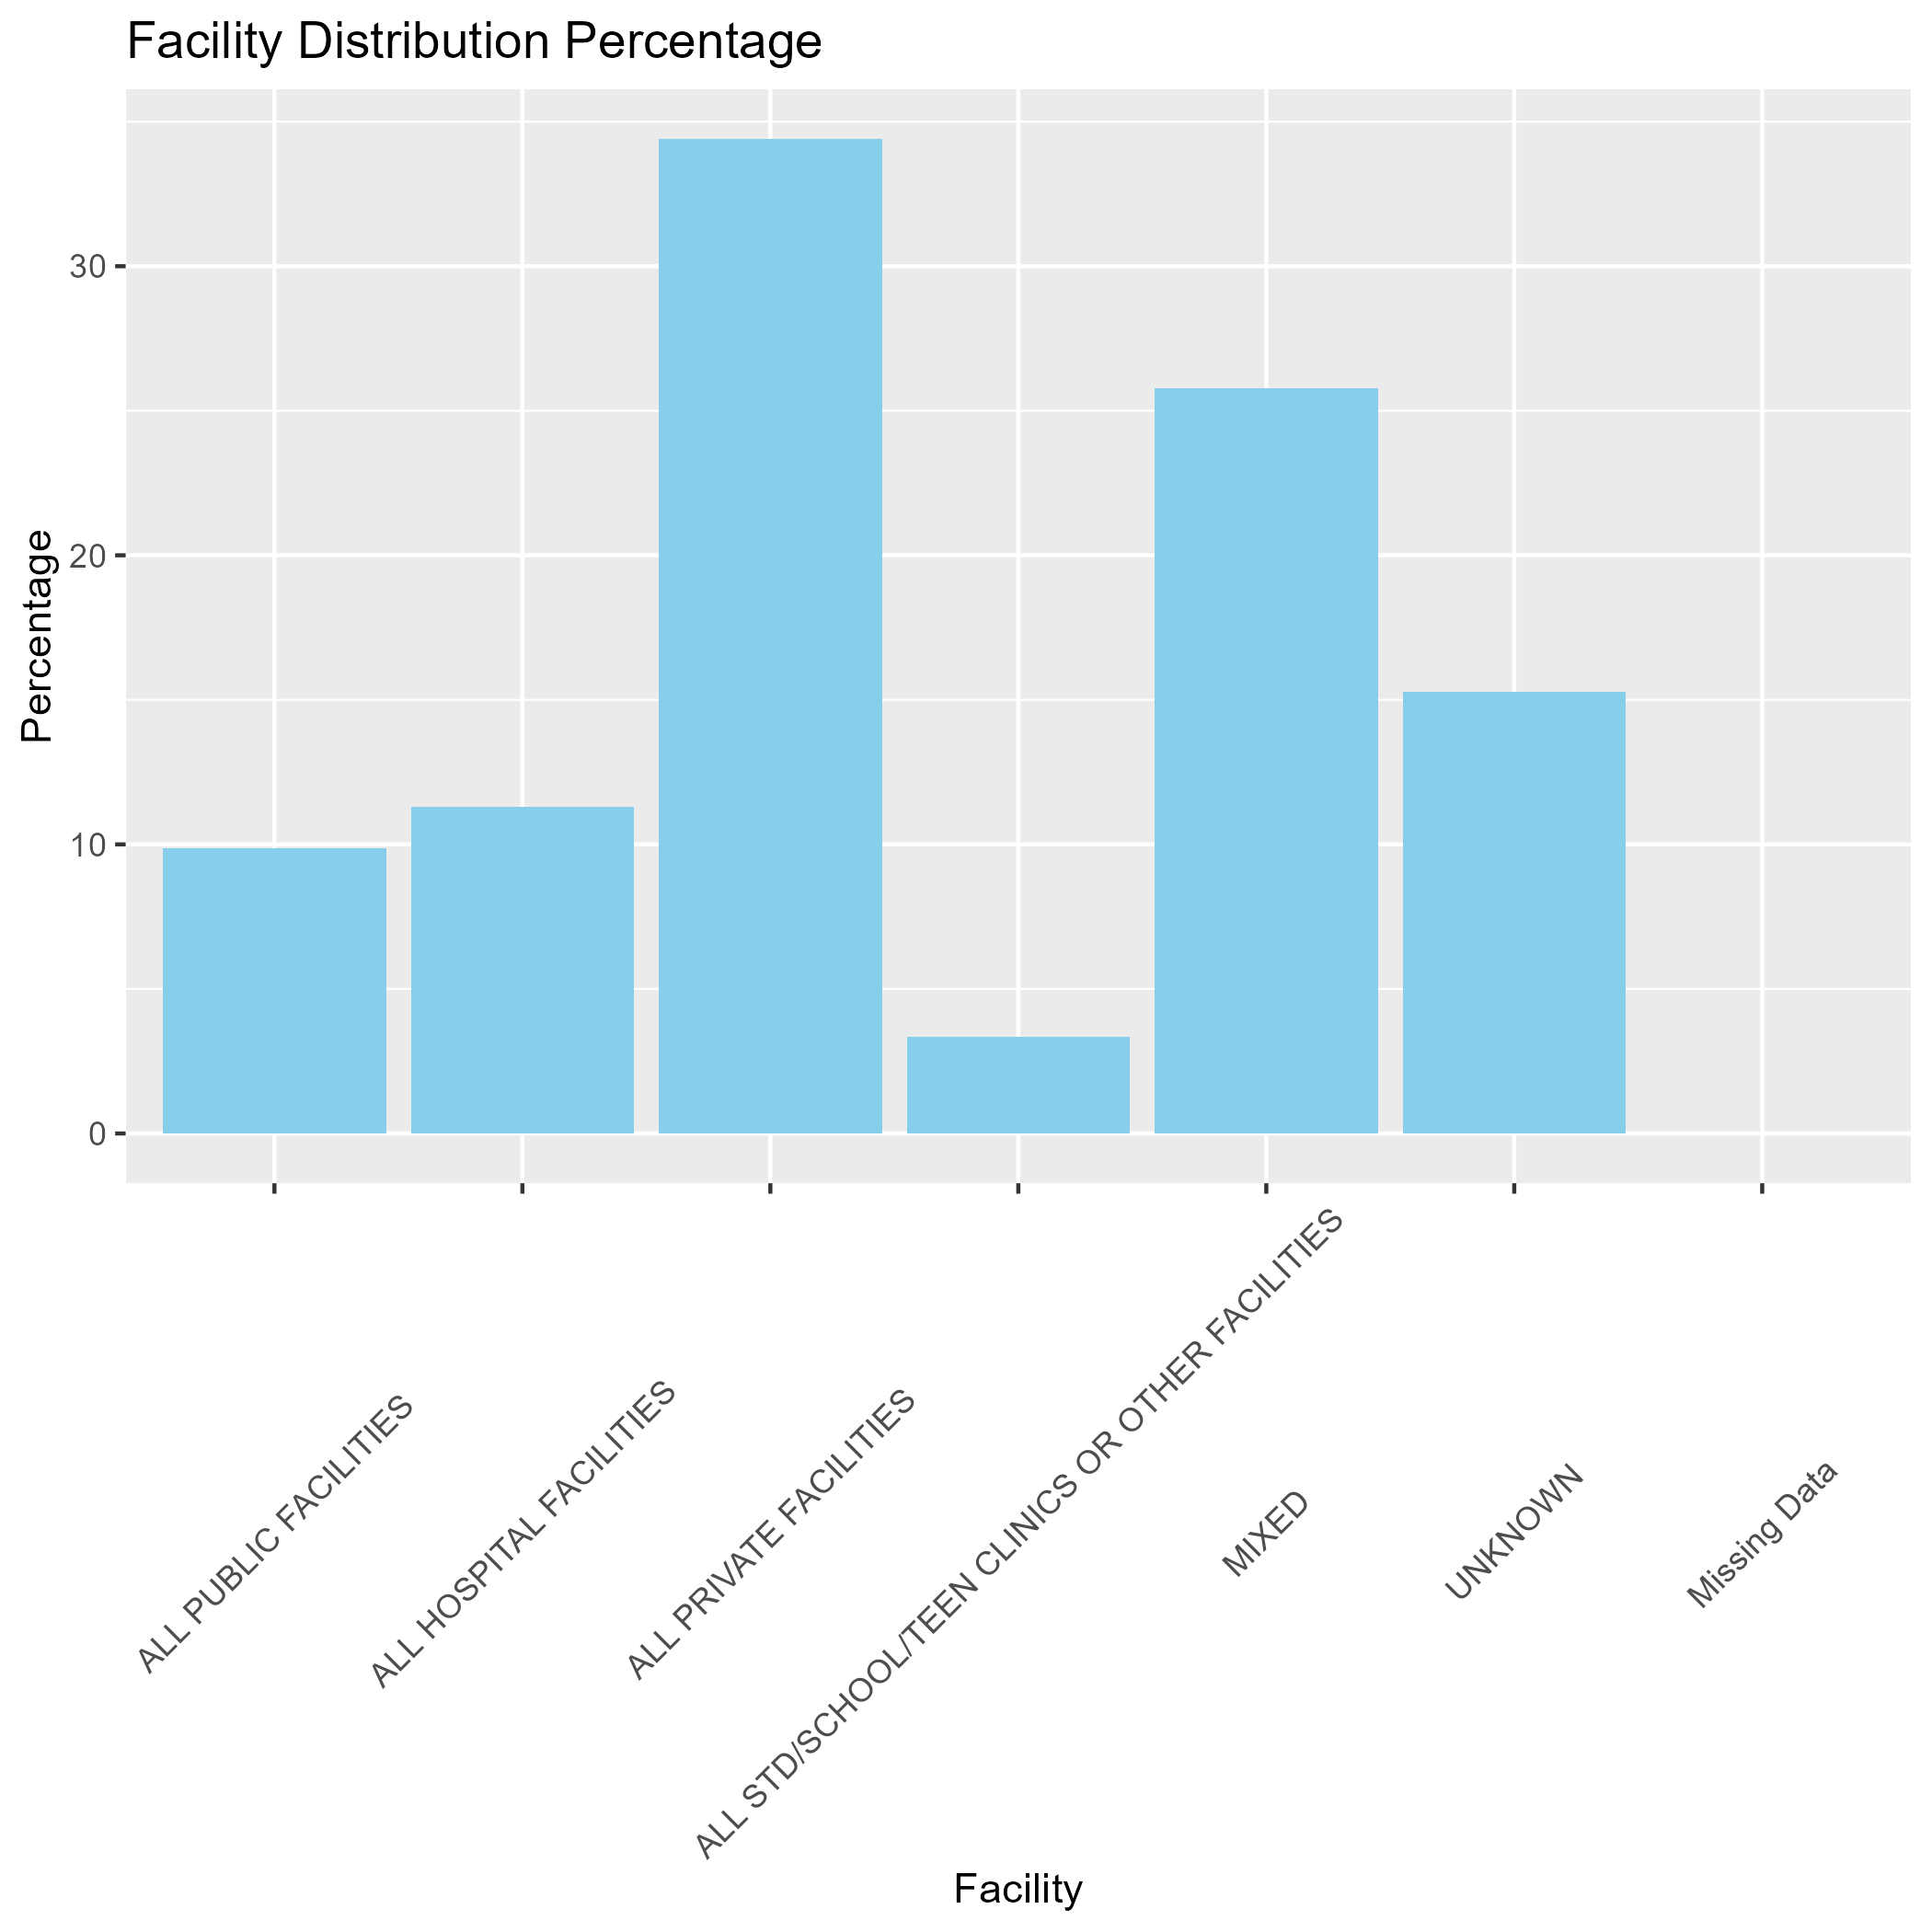
\includegraphics[width=0.8\textwidth,height=\textheight]{../../../results/figures/facility.distribution.png}
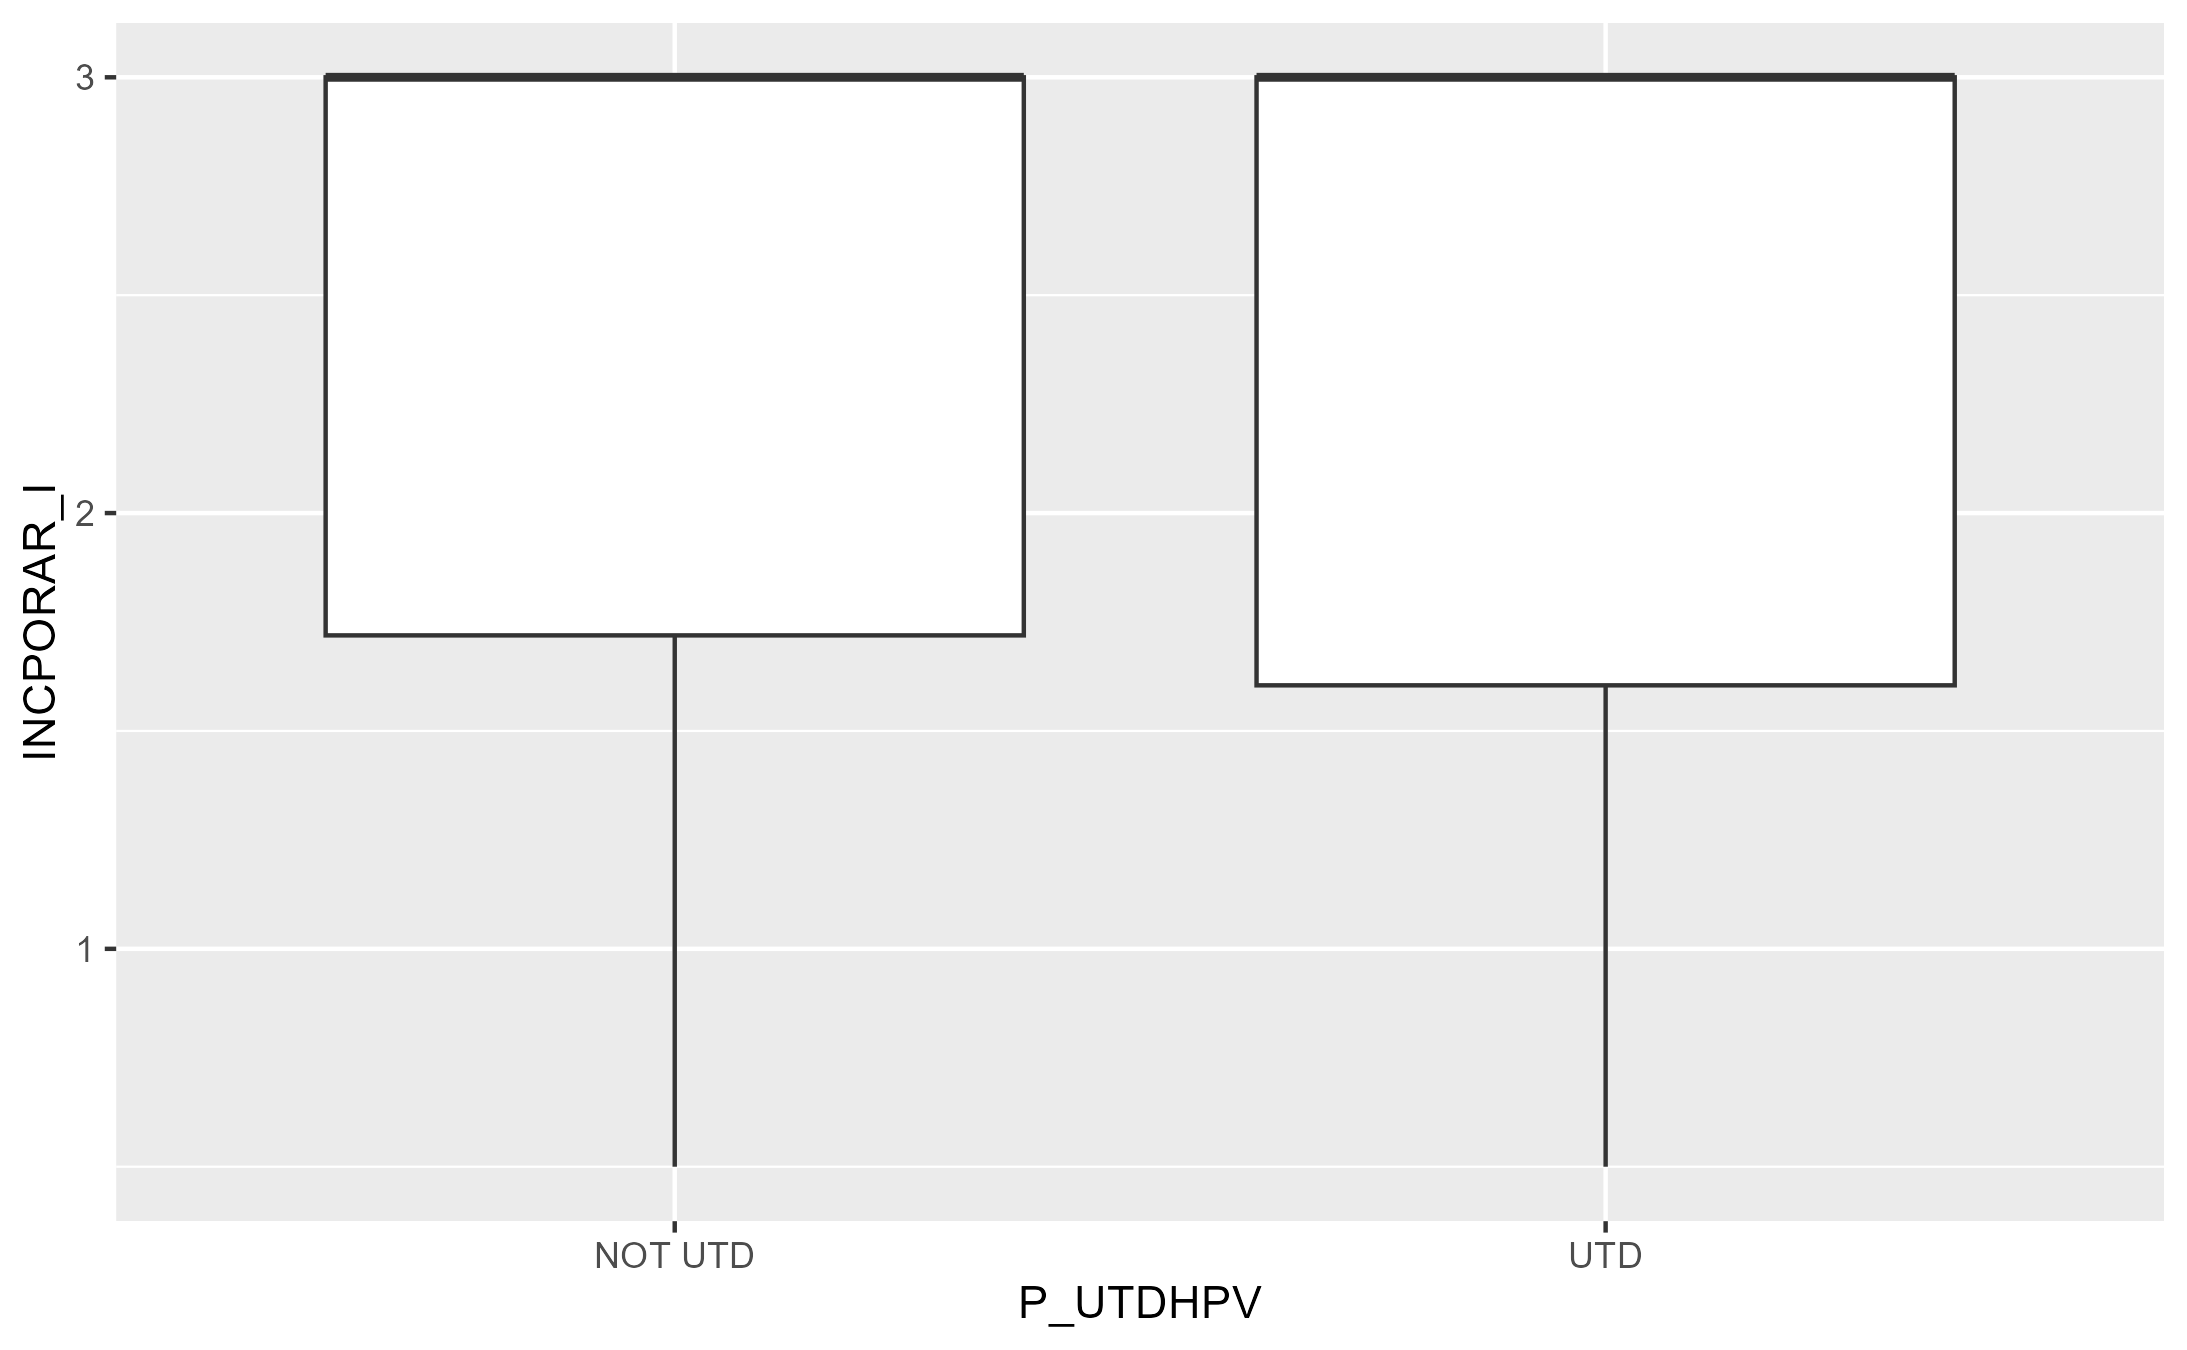
\includegraphics[width=0.8\textwidth,height=\textheight]{../../../results/figures/income-vaccination.png}

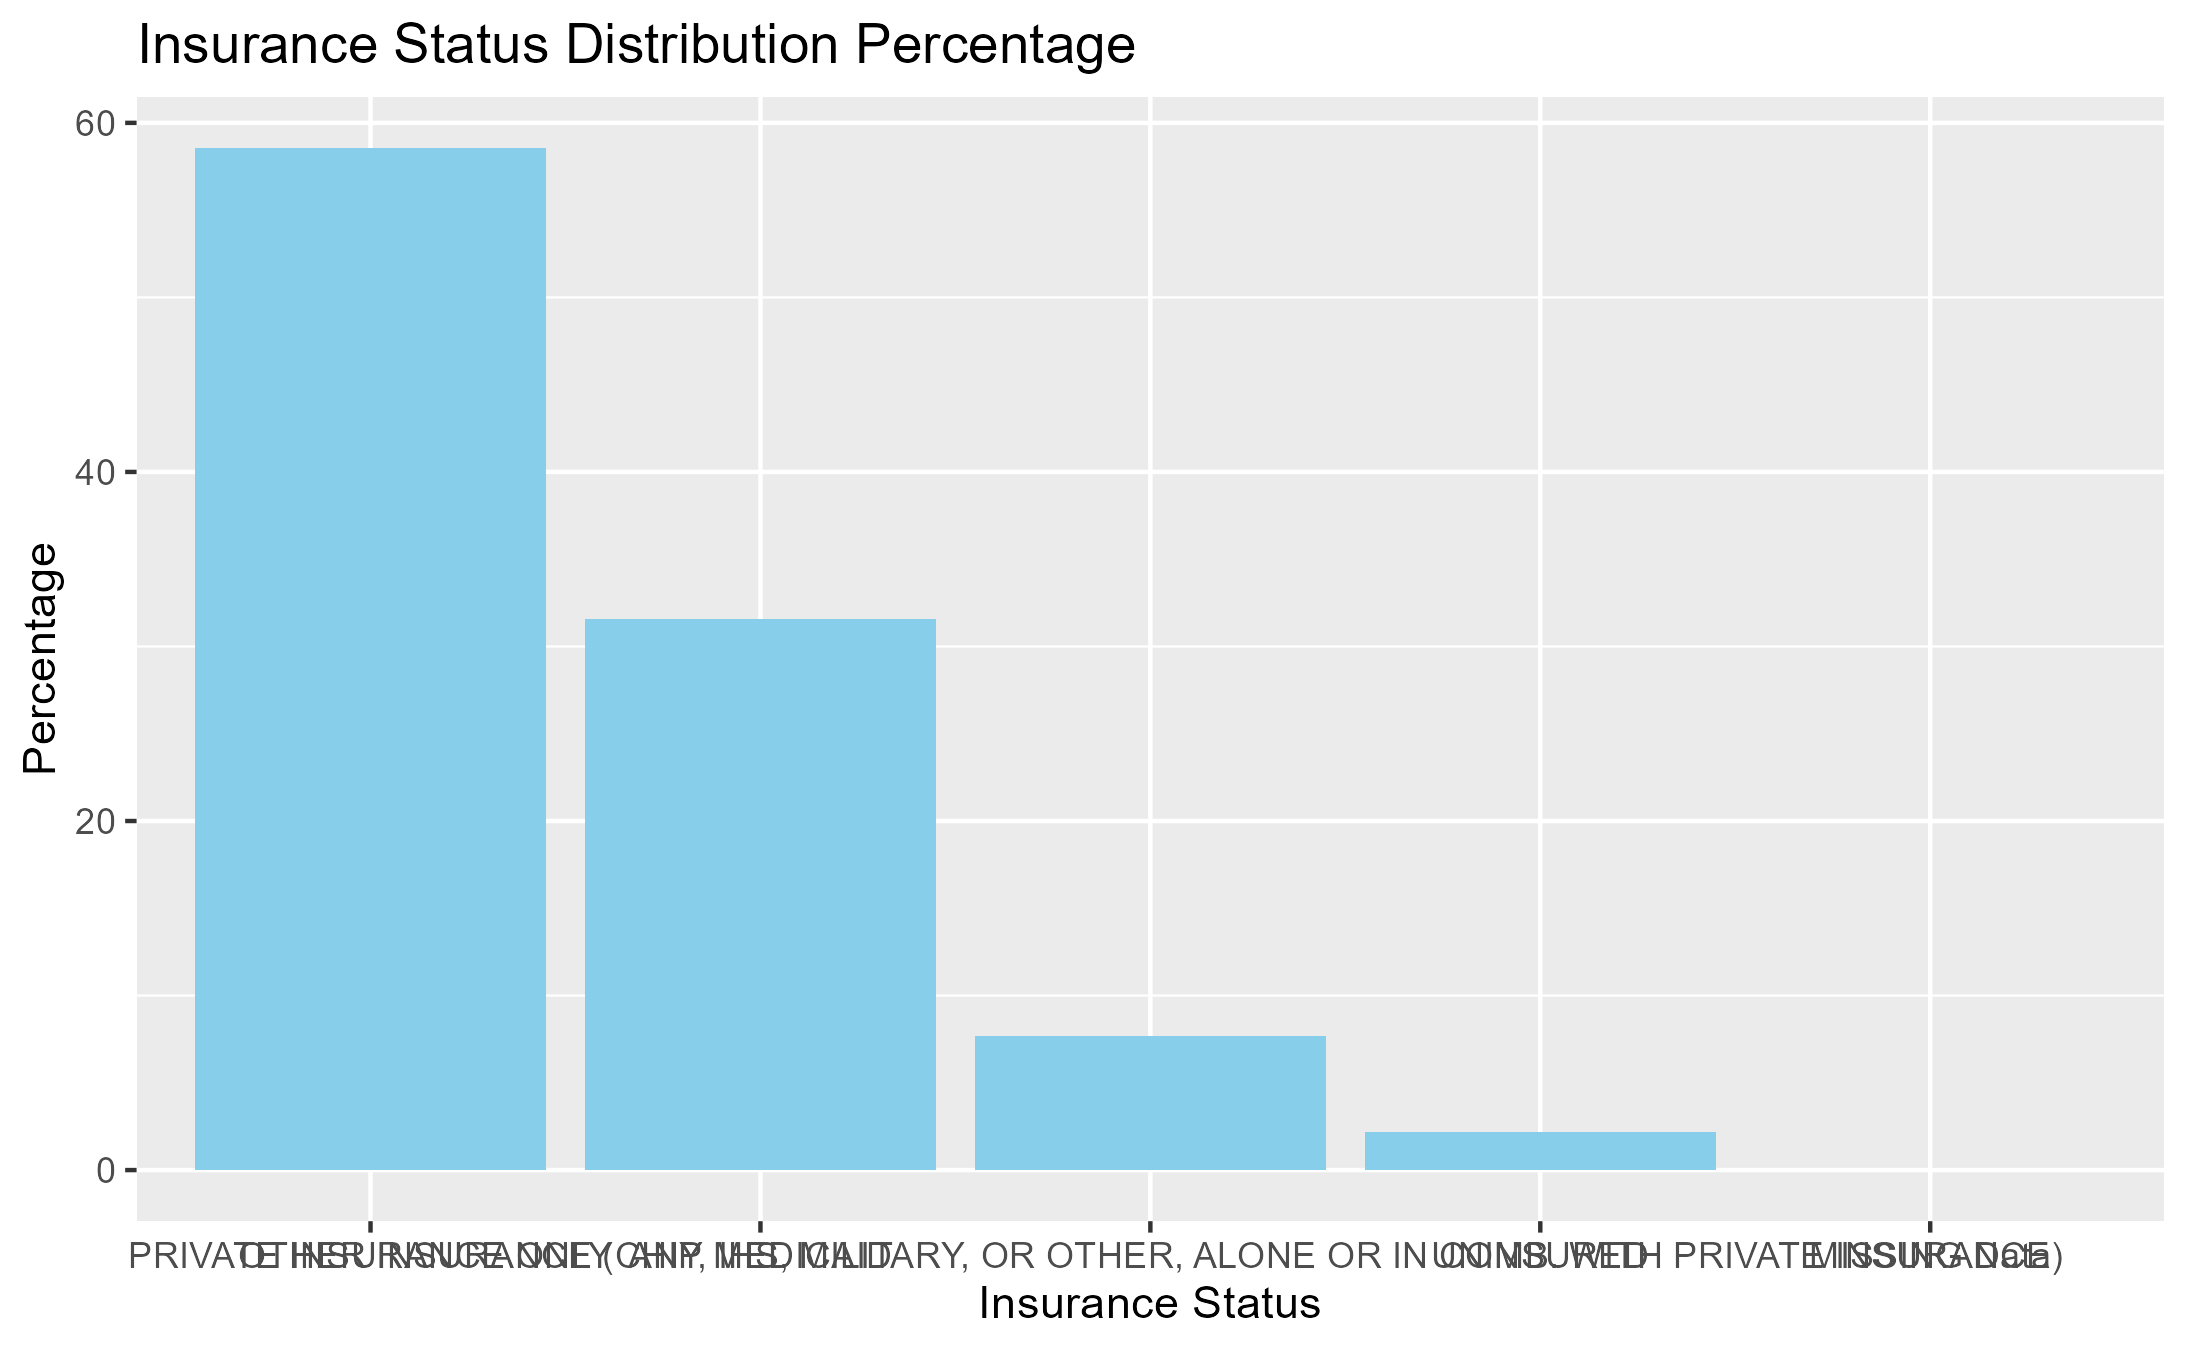
\includegraphics[width=0.8\textwidth,height=\textheight]{../../../results/figures/insurance.status.distribution.png}
\includegraphics[width=0.8\textwidth,height=\textheight]{../../../results/figures/race-ethnicity-vaccination.png}
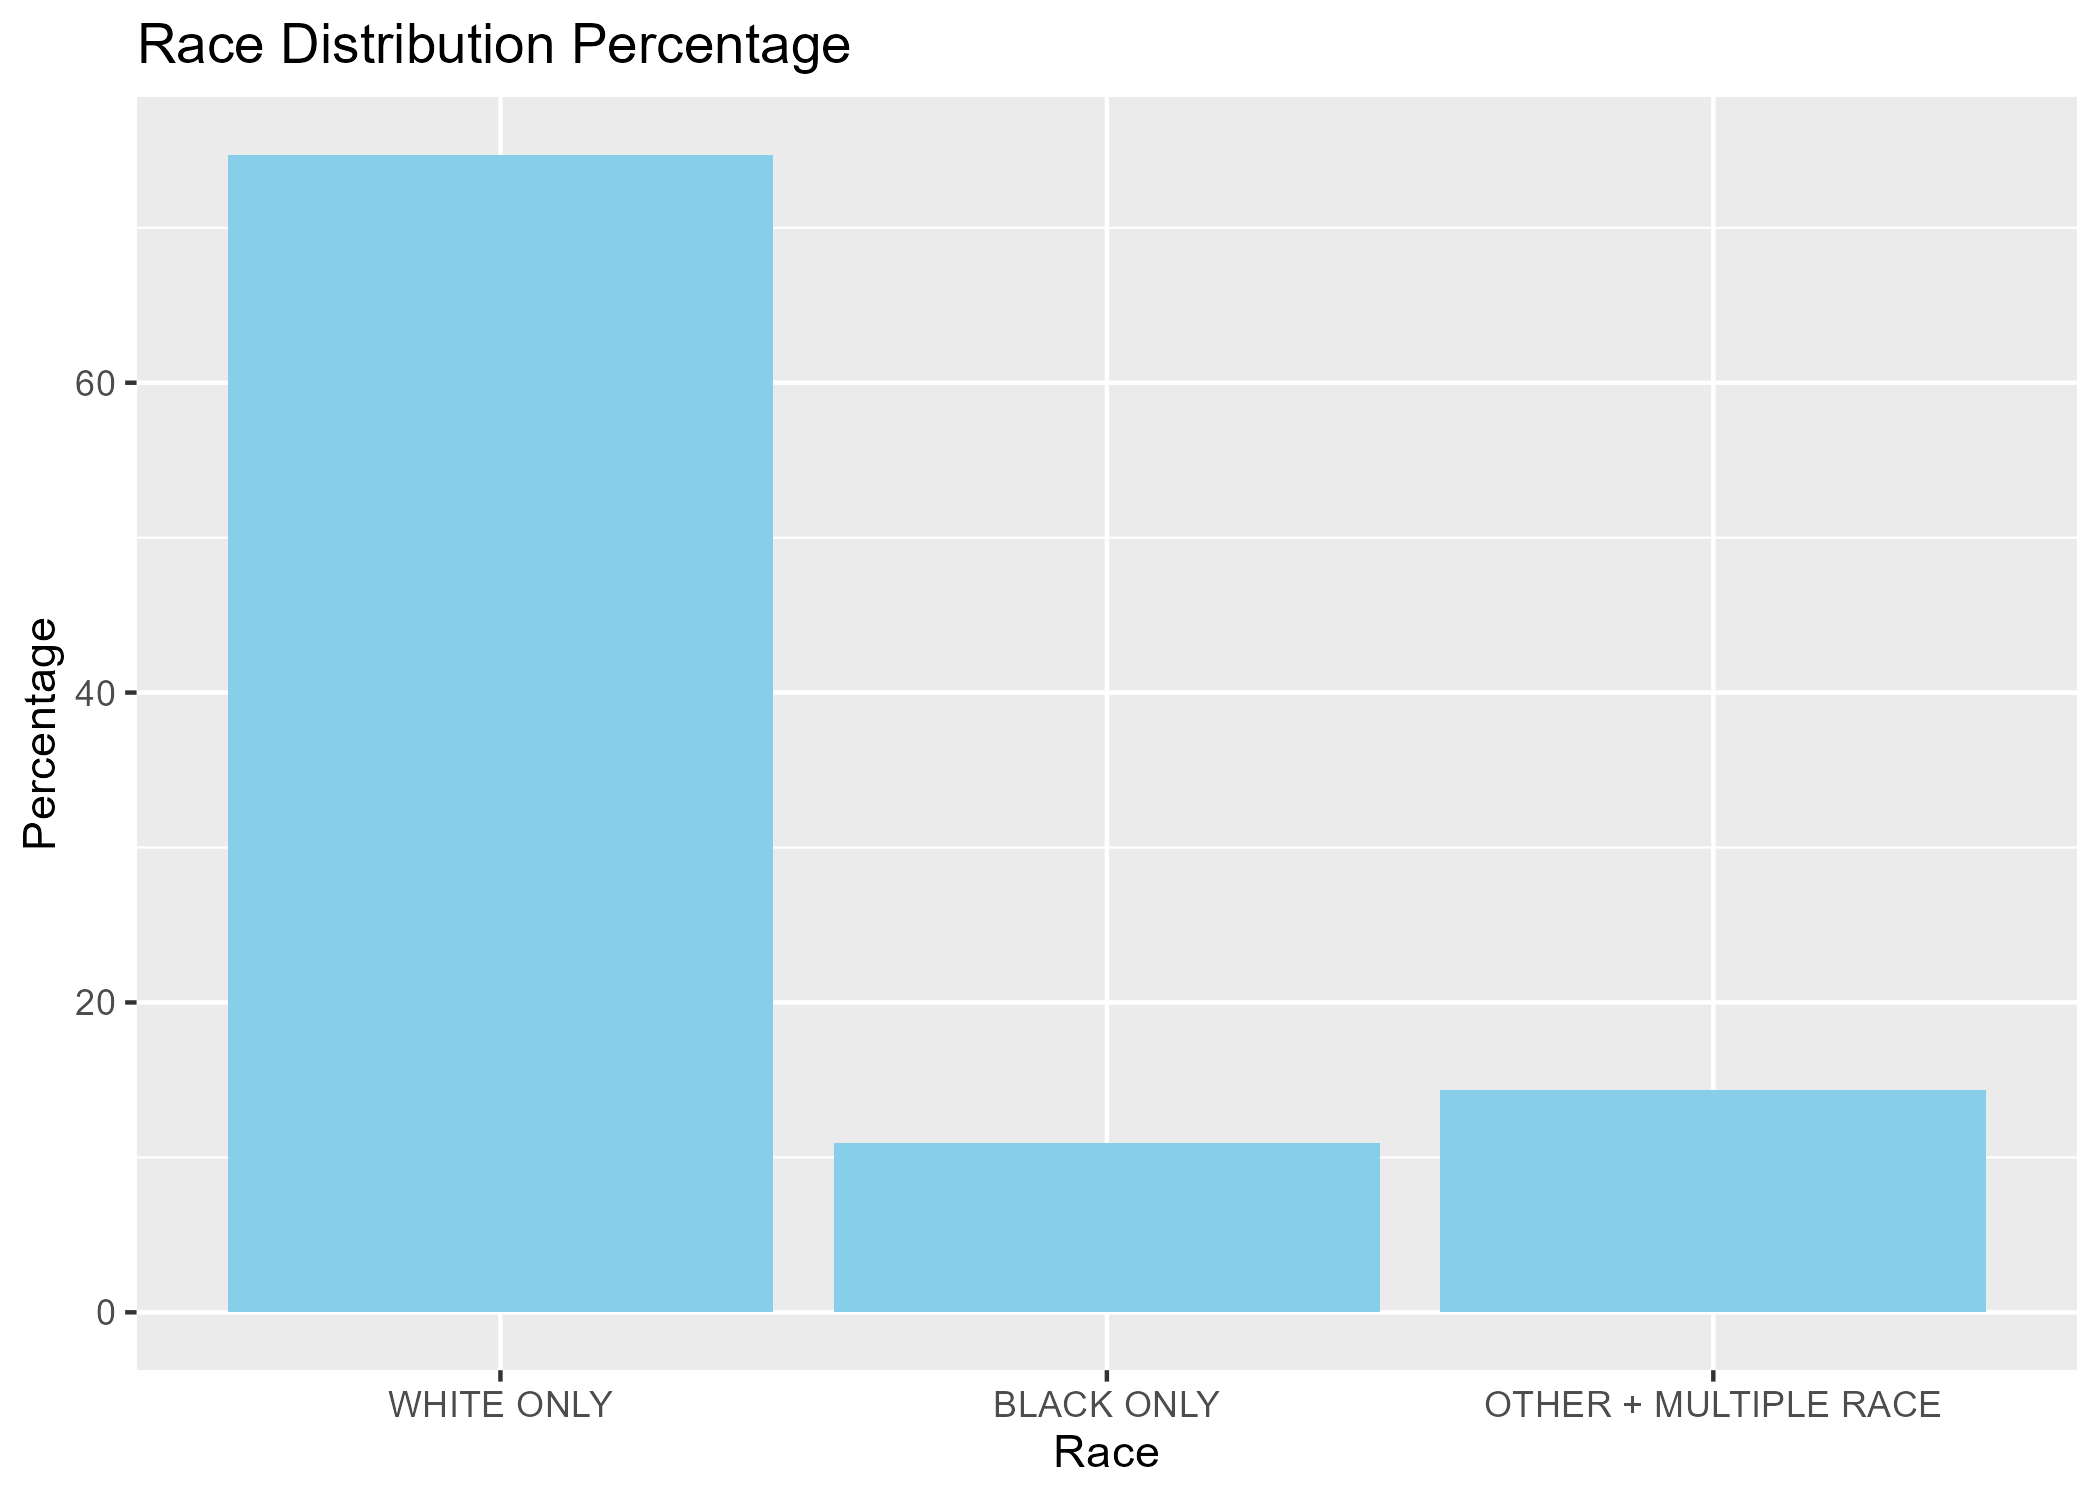
\includegraphics[width=0.8\textwidth,height=\textheight]{../../../results/figures/race.distribution.png}

\begin{figure}[H]

{\centering \includegraphics[width=0.8\textwidth,height=\textheight]{../../../results/figures/state_distribution.png}

}

\caption{S.7. The percentage of surveys submitted for each state in the
U.S. study.}

\end{figure}%%
\begin{figure}[H]

{\centering 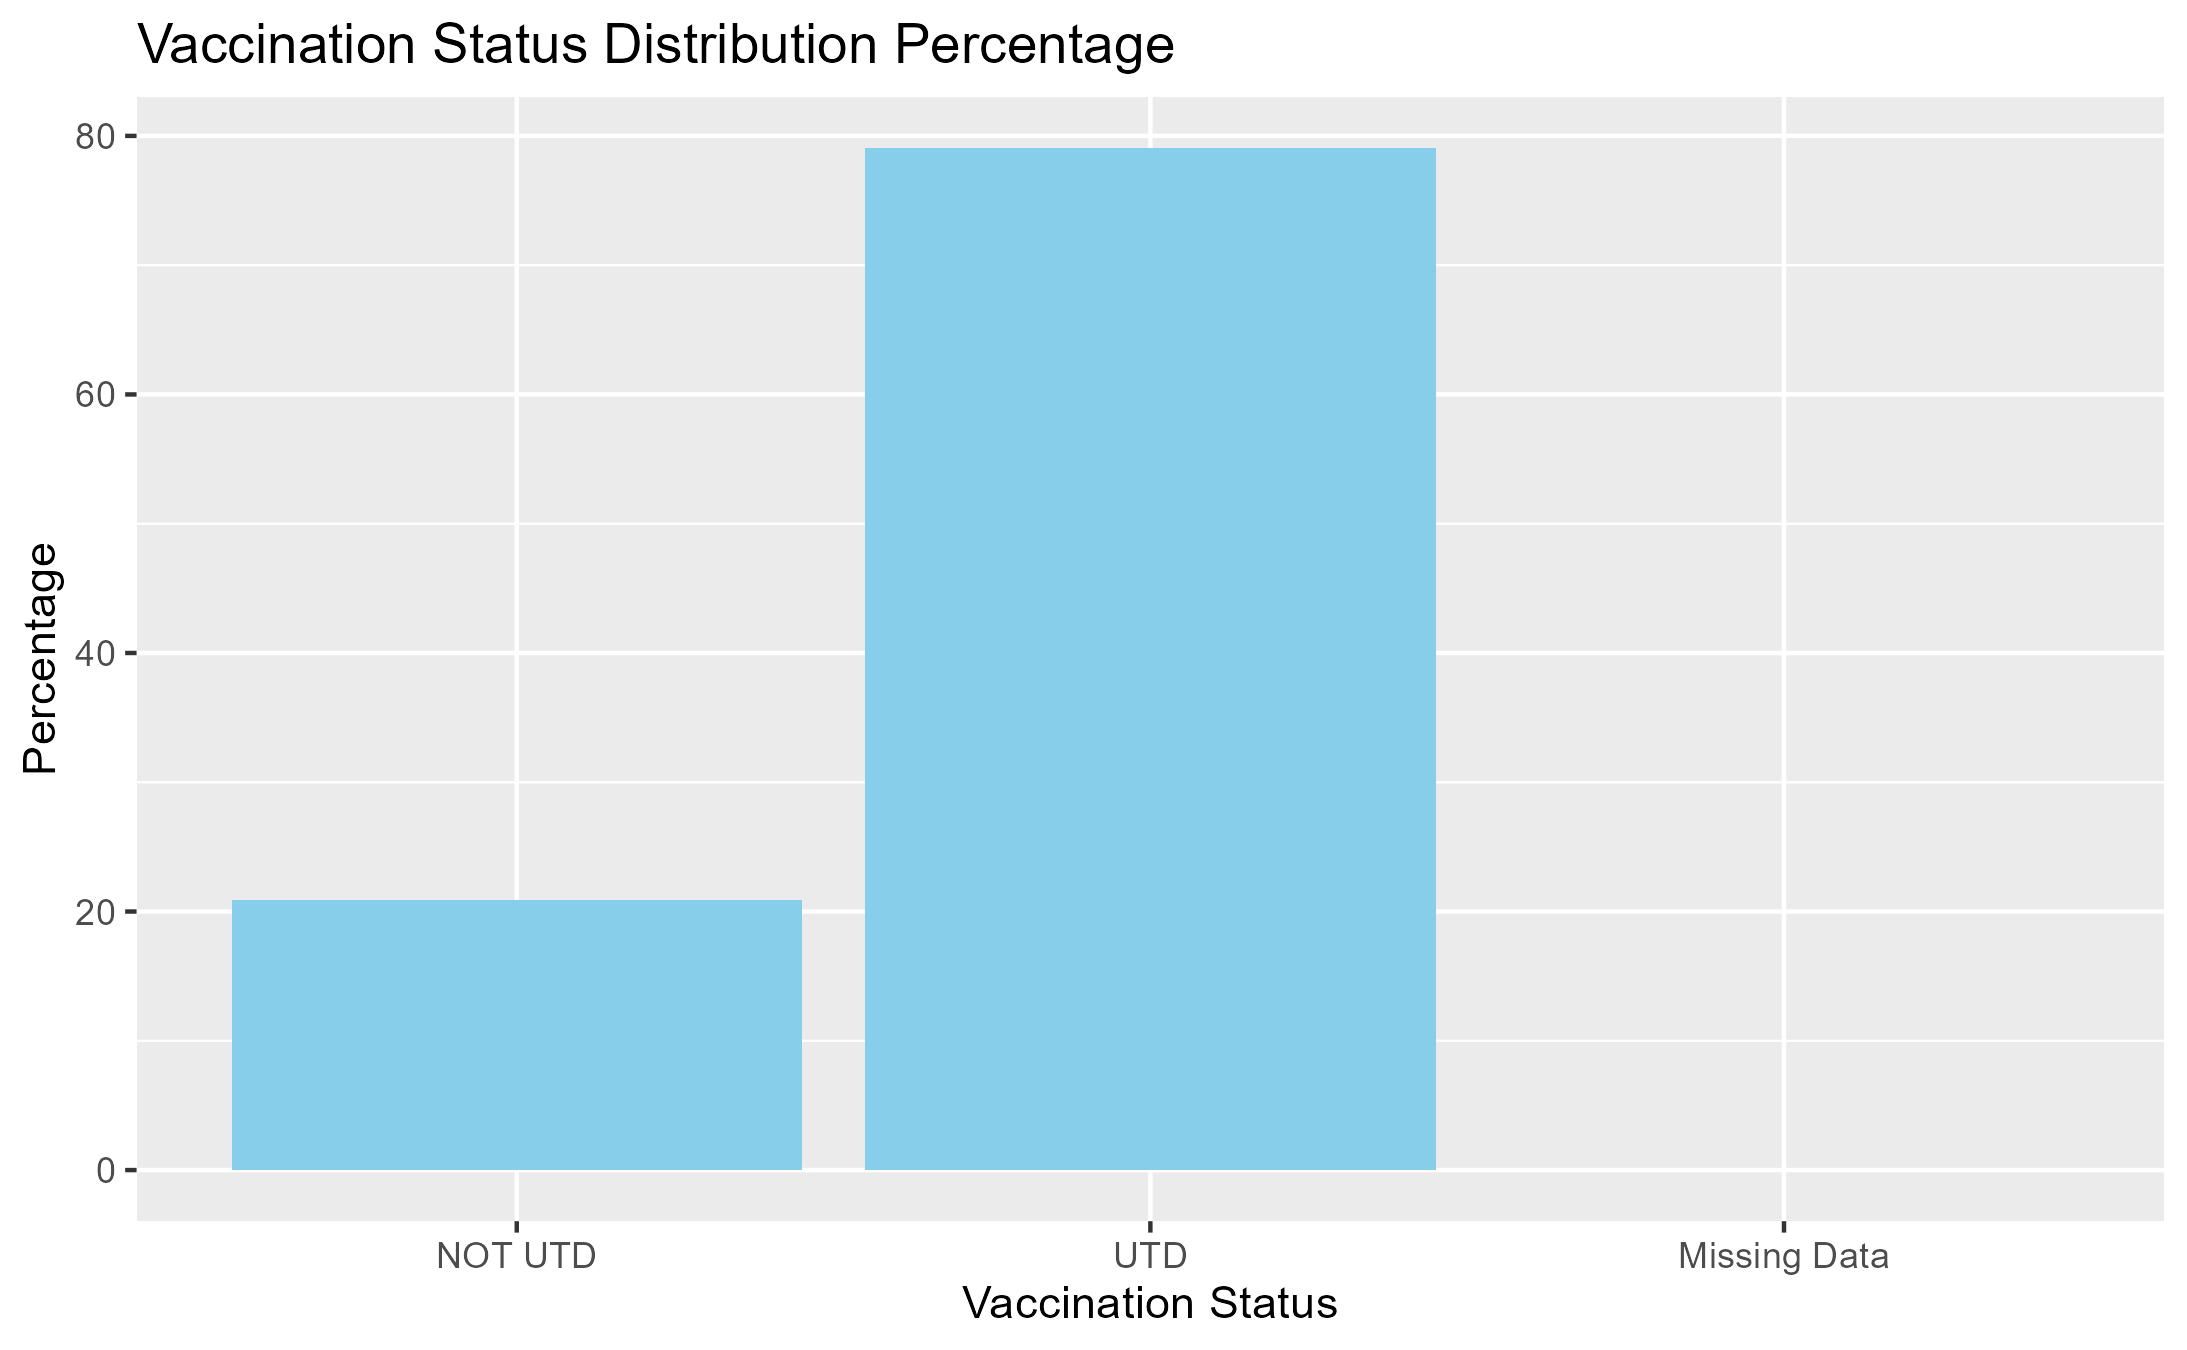
\includegraphics[width=0.8\textwidth,height=\textheight]{../../../results/figures/vaccination.status.distribution.png}

}

\caption{S.8. The distribution of HPV vaccination status in the overall
study population of U.S. teens.}

\end{figure}%%
\begin{figure}[H]

{\centering \includegraphics[width=0.8\textwidth,height=\textheight]{../../../results/figures/race-ethnicity-vaccination.png}

}

\caption{S.9. The distribution of race/ ethnicity in U.S. teens in the
study population, stratified by HPV vaccination status.}

\end{figure}%

\begin{longtable}[]{@{}lr@{}}
\caption{S.10. Percentage of up-to-date HPV vaccination status for each
state from study sample.}\tabularnewline
\toprule\noalign{}
STATE & percentage\_UTD \\
\midrule\noalign{}
\endfirsthead
\toprule\noalign{}
STATE & percentage\_UTD \\
\midrule\noalign{}
\endhead
\bottomrule\noalign{}
\endlastfoot
ALABAMA & 73.68421 \\
ALASKA & 75.21008 \\
ARIZONA & 76.02996 \\
ARKANSAS & 73.47561 \\
CALIFORNIA & 74.37500 \\
COLORADO & 81.49254 \\
CONNECTICUT & 79.29688 \\
DELAWARE & 84.80000 \\
DISTRICT OF COLUMBIA & 86.38298 \\
FLORIDA & 74.42623 \\
GEORGIA & 71.51515 \\
HAWAII & 87.98283 \\
IDAHO & 77.73279 \\
ILLINOIS & 82.82504 \\
INDIANA & 77.34375 \\
IOWA & 87.92271 \\
KANSAS & 73.85621 \\
KENTUCKY & 68.72727 \\
LOUISIANA & 79.87805 \\
MAINE & 78.65169 \\
MARYLAND & 85.21739 \\
MASSACHUSETTS & 86.51685 \\
MICHIGAN & 76.37795 \\
MINNESOTA & 85.45455 \\
MISSISSIPPI & 56.14035 \\
MISSOURI & 74.29577 \\
MONTANA & 82.35294 \\
NEBRASKA & 83.73984 \\
NEVADA & 73.72549 \\
NEW HAMPSHIRE & 85.71429 \\
NEW JERSEY & 72.98246 \\
NEW MEXICO & 81.85185 \\
NEW YORK & 81.46067 \\
NORTH CAROLINA & 75.27778 \\
NORTH DAKOTA & 85.35714 \\
OHIO & 78.81041 \\
OKLAHOMA & 70.61224 \\
OREGON & 81.39535 \\
PENNSYLVANIA & 83.06667 \\
PUERTO RICO & 86.52695 \\
RHODE ISLAND & 94.71831 \\
SOUTH CAROLINA & 75.37879 \\
SOUTH DAKOTA & 81.27490 \\
TENNESSEE & 71.12971 \\
TEXAS & 73.59694 \\
UTAH & 76.86567 \\
VERMONT & 87.93103 \\
VIRGINIA & 80.06757 \\
WASHINGTON & 81.00358 \\
WEST VIRGINIA & 70.78189 \\
WISCONSIN & 82.35294 \\
WYOMING & 69.47368 \\
\end{longtable}

\begin{longtable}[]{@{}
  >{\raggedright\arraybackslash}p{(\columnwidth - 6\tabcolsep) * \real{0.4861}}
  >{\raggedleft\arraybackslash}p{(\columnwidth - 6\tabcolsep) * \real{0.1667}}
  >{\raggedleft\arraybackslash}p{(\columnwidth - 6\tabcolsep) * \real{0.1389}}
  >{\raggedleft\arraybackslash}p{(\columnwidth - 6\tabcolsep) * \real{0.2083}}@{}}
\caption{S.11. Percentage and Count of up-to-date HPV vaccination status
according to racial and ethnic group.}\tabularnewline
\toprule\noalign{}
\begin{minipage}[b]{\linewidth}\raggedright
RACEETHK
\end{minipage} & \begin{minipage}[b]{\linewidth}\raggedleft
total\_count
\end{minipage} & \begin{minipage}[b]{\linewidth}\raggedleft
UTD\_count
\end{minipage} & \begin{minipage}[b]{\linewidth}\raggedleft
percentage\_UTD
\end{minipage} \\
\midrule\noalign{}
\endfirsthead
\toprule\noalign{}
\begin{minipage}[b]{\linewidth}\raggedright
RACEETHK
\end{minipage} & \begin{minipage}[b]{\linewidth}\raggedleft
total\_count
\end{minipage} & \begin{minipage}[b]{\linewidth}\raggedleft
UTD\_count
\end{minipage} & \begin{minipage}[b]{\linewidth}\raggedleft
percentage\_UTD
\end{minipage} \\
\midrule\noalign{}
\endhead
\bottomrule\noalign{}
\endlastfoot
HISPANIC & 3303 & 2728 & 82.59158 \\
NON-HISPANIC WHITE ONLY & 9738 & 7514 & 77.16163 \\
NON-HISPANIC BLACK ONLY & 1516 & 1218 & 80.34301 \\
NON-HISPANIC OTHER + MULTIPLE RACE & 2007 & 1639 & 81.66418 \\
\end{longtable}



\end{document}
